%*****************************************************************************************
\part{Analysis of Current System}
\chapter{Introduction and Background}
\ifpdf
    \graphicspath{{Chapter2/Figs/Raster/}{Chapter2/Figs/PDF/}{Chapter2/Figs/}}
\else
    \graphicspath{{Chapter2/Figs/Vector/}{Chapter2/Figs/}}
\fi

%%%%%%%%%%%%%%%%%%%%%%%%%%%%%%%%%%%%%%%%%%%%%%%%%%%%%%%%%%%%%%%%%%%%%%%%%%%%%%%
\section{Introduction}

This part of the project can be outlined as follows:

\begin{itemize}
    \item Collect data sets on which a machine learning classifier is to be trained
    \item Construct a program capable of processing and storing such data sets
        such that required subsets of the data can be quickly and easily
        returned for further analysis
    \item Select a suitable machine learning framework to handle the training
        and validation of a classifier
    \item Ensure a robust validation methodology exists for assuring quality of
        our own results
    \item Set up an environment capable of allowing results from such a
        classifier to be stored and compared
    \item Training a suitable classifier on the collected data sets
    \item Perform experiments by selecting subsets of the variables and
        observations and measure whether classification accuracy is improved
\end{itemize}


%%%%%%%%%%%%%%%%%%%%%%%%%%%%%%%%%%%%%%%%%%%%%%%%%%%%%%%%%%%%%%%%%%%%%%%%%%%%%%%
\section{Concepts and Terminology}
\subsection{DNA and Bases}

...DNA is made up of four bases; G, C, T and A...

\subsection{Next Generation Sequencing}

...the process of recovering or extracting the sequence of nucleotide bases...

\subsection{Single Nucleotide Polymorphisms}

...SNPs...

\subsection{Samples, Lanes and Lanelets}
\label{chap:samplelanelanelets}

%TODO Draw a vector of the lanelets diagram
%TODO Illumina DNA Synthesis Image
A \textbf{sample} is a distinct DNA specimen extracted from a particular person.
For the purpose of sequencing, samples are pipetted in to a \textit{flowcell}
such as the one in Figure~\ref{fig:flowcell} -- a glass slide
containing a series of very thin tubules known as \textbf{lanes}.  It is
throughout these lanes that the chemical reactions involved in sequencing take place.

\begin{figure}[htbp!]
    \centering
    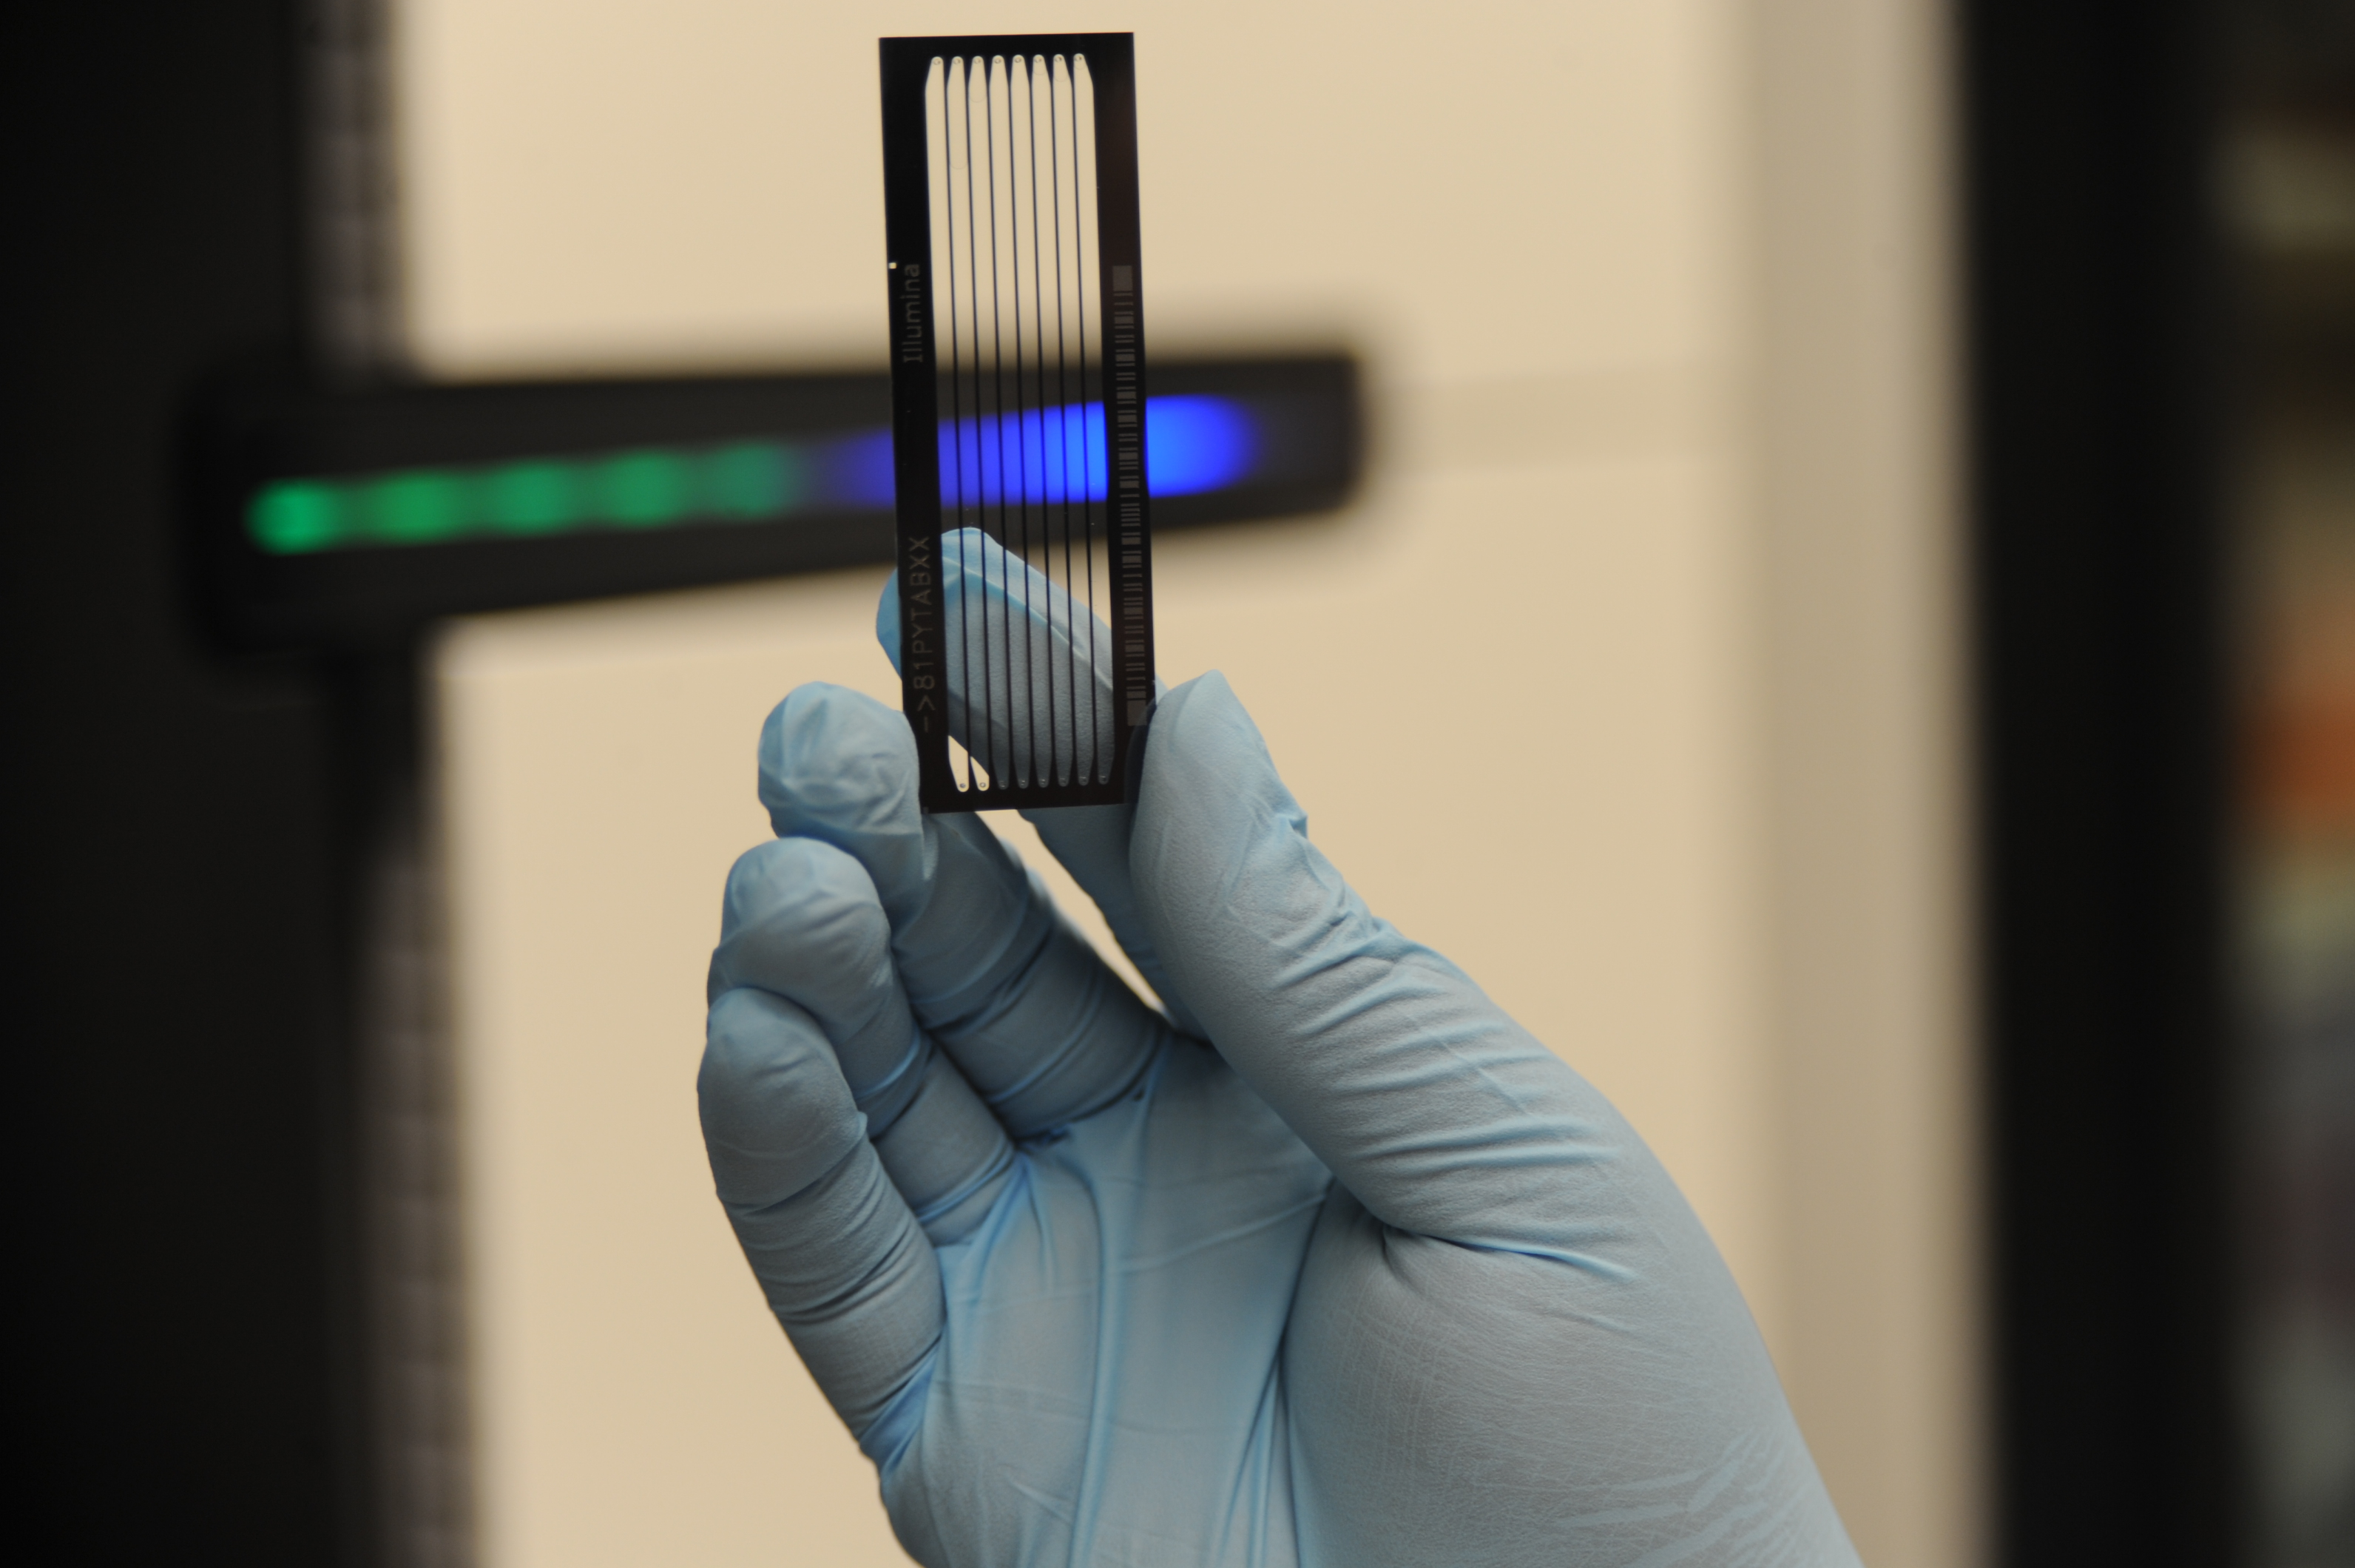
\includegraphics[width=0.4\textwidth]{NHGRI-80102}
    \caption[flowcell]{An Illumina HiSeq Flowcell\citep{img:flowcell}}
    \label{fig:flowcell}
\end{figure}

Once inserted, samples are amplified \textit{in situ}, in the flowcell itself. A
process in which the genetic material of each sample is caused to multiply in
magnitude to form a dense cluster of the sample around the original. Millions of
clusters will be created throughout each lane of the flowcell.

Note that a lane can contain more than one sample and a sample can appear in
more than one lane; this is known as \textit{sample multiplexing} and helps to
ensure that the failure of a particular lane does not hinder analysis of a
sample (as it will still be sequenced as part of another lane).

%TODO Describe lanelet as a Sanger coined term

The more abstract of the definitions, a \textbf{lanelet} is the aggregate read
of all clusters of a particular sample in a single lane.
Figure~\ref{fig:lanelets} attempts to highlight examples of a this (circled in
blue -- not all lanelets are highlighted). For example Lane 5 shows the four
clusters (in reality there would be millions) of Sample A combine to
represent a lanelet. A lane will have as many lanelets as it does samples.

%TODO Describe lanelet ID

\begin{figure}[htbp!]
    \centering
    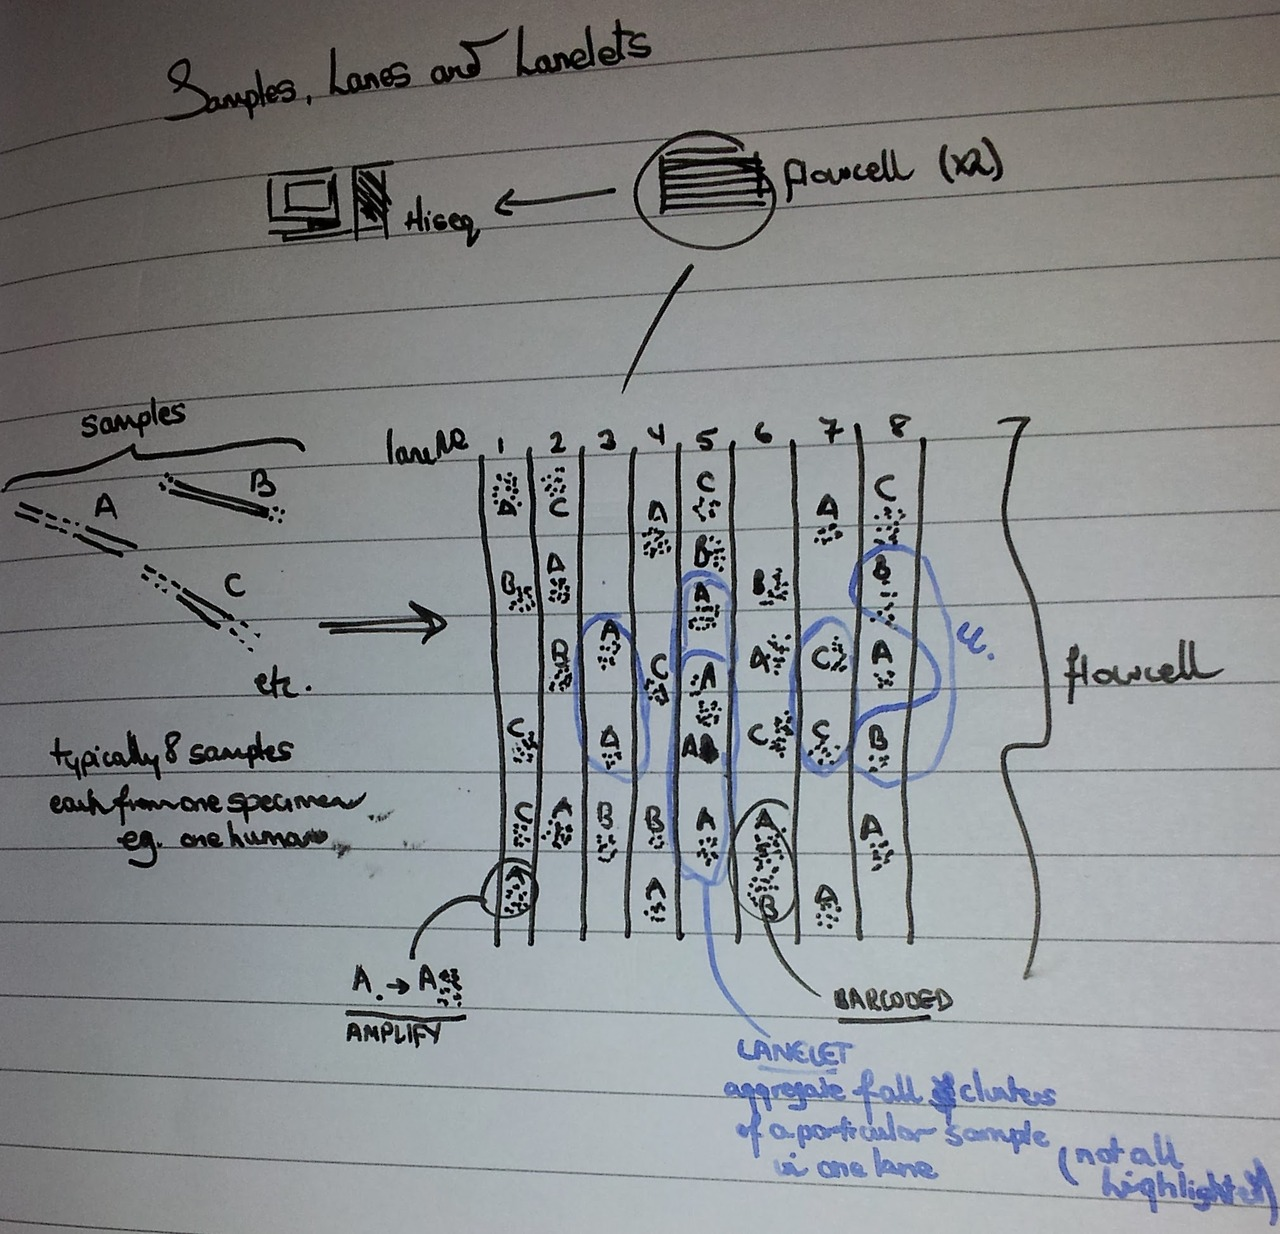
\includegraphics[width=0.5\textwidth]{lanelets}
    \caption[lanelets]{Example of flowcell with some lanelets highlighted}
    \label{fig:lanelets}
\end{figure}


%%%%%%%%%%%%%%%%%%%%%%%%%%%%%%%%%%%%%%%%%%%%%%%%%%%%%%%%%%%%%%%%%%%%%%%%%%%%%%%
\chapter{Materials and Methods}
\section{Input Data and Format}
\subsection{"BAMcheckR'd" Data}
\label{chap:bamcheckr-data}

%NOTE Assuming lanelets have been described by this point...
%TODO samtools stats actually generates this data rather than "the seq process"
As part of the project I have been granted access to significant data sets at the
Sanger Institute, unlocking quality control data for two of the largest studies
currently undergoing analysis. A wide array of quality metrics are available for
each and every lanelet that forms part of either of the two studies, totalling
13,455 files.
%TODO Cite and explain the security policy for this data

%9154 (68\%), 1542 (11\%), 2759 (21\%)...

%TODO Explain a BAM file
The files are created by \textbf{samtools stats} -- part of a collection of
widely used open-source utilities for post-processing and manipulation of large
alignments such as those produced by next-generation sequencers that are
released under the umbrella name of "SAMtools"\citep{samtools} (Sequence
Alignment and Map Tools). \textbf{samtools stats} collects statistics from
sequence data files and produces key-value summary numbers as well as more
complex tab delimited dataframes tabulating several metrics over time.

%TODO Was samtools stats known as bamcheck, or did it replace it?
The output of \textbf{samtools stats} is then parsed by an in-house tool called
\textbf{bamcheckr}\footnote{Named such as \textbf{samtools stats} now incorporates
\textbf{bamcheck} and the tool is written in R} which supplements the summary
numbers section of the \textbf{samtools stats} output with additional metrics
that are later used by \textbf{auto\_qc} for classification.  This process
appends additional key-value pairs in the summary numbers section.  A truncated
example of a "bamcheckr'd" file can be found in Appendix~\ref{app:bamcheckr}.

It is these summary numbers that will be the main focus of our learning task.


\subsection{auto\_qc Decision Data}

To use these "bamcheckr'd" files for training and testing a machine learning
classifier, it is necessary to map each file to a classification result from
\textbf{auto\_qc}. The one-to-one mapping between each input file and its label
are provided by the Sanger Institute in a separate file hereafter referred to as
the \textit{AQC Decision Matrix} or \textit{AQC (Decision) File}.

A truncated example of such a file can be found in
Appendix~\ref{app:aqc_matrix}.  Only the first few columns are included --
indeed we are only interested in the \textit{lanelet} and \textit{aqc} fields
which provide an identifier that maps the row to a given input file and its
classification by \textbf{auto\_qc} respectively.  Latter columns pertain to a
breakdown of decisions made by \textbf{auto\_qc} which are not included in the
example for confidentiality (and brevity).


%%%%%%%%%%%%%%%%%%%%%%%%%%%%%%%%%%%%%%%%%%%%%%%%%%%%%%%%%%%%%%%%%%%%%%%%%%%%%%%
\section{Development Environment}
\subsection{Language}
\label{part1:dev:lang}

%TODO Better opening
%TODO Do I need to ramble about why vim is great and so on?
Python was selected for the language of the program designed to handle this vast
array of input data, more out of personal taste rather than a detailed analysis
of required performance and features. From previous experience I was happy with
the performance of Python when processing large datasets in terms of both
file handling operations and storing the data in memory for later use. Python's
generous choice of both built-in and third-party libraries have proven useful.
Due to its concise and flexible nature it is possible to rapidly
develop applications and its readability eases ongoing maintenance; useful given
the short time-span allocated for this project and the possibility of others
wishing to contribute to the project codebase after completion.

Whilst the choice was made primarily on preference, this is not to say other
options were not considered: a highly popular Java-based collection of data
mining tools, \textbf{WEKA}\citep{weka} would certainly have provided a
framework for building decision tree classifiers but did not
appear to offer any significant features that were unavailable elsewhere, whilst
Java itself has the added constraint of requiring a virtual machine to be
installed which could be undesirable from a performance or security
standpoint when the application is deployed to servers at the Sanger Institute.

%...although performance has improved considerably from previous Java versions\citep{Bouckaert}

Difficulty was also encountered finding example implementations for \textbf{WEKA}
with most documentation and tutorials providing information for performing
analysis via the graphical "Explorer" interface instead, which would not be
appropriate for quickly setting up and repeating experiments automatically.

Given the quality data we'll be using to train a machine learning classifier is
output from the previously mentioned R script, \textbf{bamcheckr}, it was worth
briefly investigating the options available for R itself as the potential of
integrating the learning and predicting functions right in to the same process
that outputs the data seemed convenient.

Whilst the \textbf{tree}\citep{man:rtree} and \textbf{rpart}\citep{man:rpart}
packages are available for constructing decision trees in R (and actually
\textbf{RWeka} provides an R interface to \textbf{WEKA}) neither appeared to be
as robust as other more well-known frameworks. Also putting it politely, the
programming paradigm of R\citep{man:R} is rather different to other languages
and can significantly increase development time (and frustration\citep{argh}) if
one is not well versed in the patterns and grammar of the language  and it
seemed best to stick to one's comfort zone given the brief timescale for the
project.

Had performance been a critical decision factor, lower level languages such as
C, C++ or even Fortran could be used. Briefly looking at frameworks available
for C++ in particular, two popular solutions include: \textbf{dlib}\citep{dlib},
which did not support tree-based classifiers but did offer implementations of
other potentially useful algorithms such as multi-class support vector machines;
and \textbf{Shark}\citep{shark}, which supported both decision tree and random
forest classifiers. Both packages also provided a series of utility functions
for performing mathematical or statistical operations on vectors of data.


\subsection{Framework}

Having studied the \textit{Machine and Intelligent Learning} module in my final
year, the prospect of getting stuck in to the deep of a machine learning
algorithm was exciting. However the reality is a lot of cumulative time and
effort has gone in to the creation and optimisation of a framework, which is
unlikely to be surpassed successfully by a short-term one-person project. Thus
utilisation of a third party machine learning library seems a wise investment
for the project's codebase.

There are clearly numerous machine learning frameworks available in many
languages, some of which were touched upon in the previous section and formed
part of the development environment decisions.
Whilst it is obviously unnecessary to select a framework which uses
the same language as the project, it seemed counter-intuitive to select otherwise,
for the establishing of additional arbitrary output and input steps to move data
between the two environments could impede prompt experiment repeatability and
introduce error.

A mixed bag of machine learning frameworks exist in Python\citep{py:for-ai},
ranging from several highly active general purpose libraries to a multitude of
smaller projects that focus on one specific learning task.

I investigate two of the larger libraries;
\textbf{scikit-learn}\citep{scikit-learn} and \textbf{Orange}\citep{orange},
primarily as their general purpose nature will allow exploration of various
classifier solutions (given time) without the need to integrate many packages
together, but also for their built-in functionality that aids the measuring of
classifier performance and accuracy. These two packages were also selected for
investigation on their recommendation from the project supervisor.


\textbf{scikit-learn} is somewhat the "new kid on the block" in terms of machine
learning packages for Python, originally starting as a Google Summer of Code
project in 2007 under the name of \textbf{scikits.learn}\footnote{Named as a
\textbf{SciPy} Toolkit for Learning Tasks} the package was not officially
published until 2010 where it quickly gained popularity and built an
international team of contributors\citep{about-scikit-learn}.

Arguably one of the most useful features of \textbf{scikit-learn} is its
seamless integration with the "big names" of scientific computing in Python:
\textbf{NumPy}\citep{NumPySciPy} and \textbf{SciPy}\citep{SciPy}, making heavy
use of the optimised data structures and mathematical algorithms these packages
offer, not only providing improved performance against packages that implement
their own structures but also easing interaction by not requiring users to
populate abstruse structures with their data or implement such algorithms
themselves.

\textbf{scikit-learn} offers support for a wide range of algorithms covering
many different machine learning tasks, including decision trees and random
forests. Also of interest are the various utility subpackages, taking particular
note of one for measuring the performance of the various classifiers;
including functions for executing cross-validation and generating confusion
matrices; and another which assists with the selection of parameters (features)
to use in a machine learning model.

The library boasts a growing community of users and a dedicated team of
developers\footnote{Some full time developer positions are funded by
\textit{INRIA}, the French Institute for Research in Computer Science and
Automation} who submit hundreds of commits to the project repository each month
according to Github Pulse.


\textbf{Orange}, like \textbf{scikit-learn} is designed to be a general purpose
machine learning framework and provide a wide array of tools to work with many
different types of problems. Setting it apart from many of the other packages is
the inclusion of a graphical user interface (GUI) that presents
drag-and-drop-eqsue access to widgets from which users assemble a workflow to
apply to their data. The GUI also allows visualisation of elements such as
decision trees or confusion matrix plots without any effort from the end user.

Despite the repository commit history stretching back to mid 90s, only recent
improvements including a major redesign of the GUI, significant changes to
its object hierarchy and its 2013 academic publication have brought more
attention to the framework.

At first glance \textbf{Orange} appears to offer a larger collection of
functions to work specifically with classification tasks when compared to
\textbf{scikit-learn}. Indeed it would later be discovered that it ships with
features useful to the project that have not been implemented in
\textbf{scikit-learn} including tree pruning and printing.

However it does not feature the same integration with
Python's scientific computing packages; \textbf{NumPy} and \textbf{SciPy} and
also requires that end users input their data in a structure defined by
the framework rather than a generic data structure.
Thus use of \textbf{Orange} would introduce more data wrangling and munging
steps to ensure that data is represented in the correct format for a classifier
to perform its learning and prediction role and also to interpret returned objects.

Although \textbf{Orange} affords a suitable (and in some cases better) range of
functions to use for decision trees, I was concerned at the push to use its GUI
as opposed to the package API, potentially impeding experiment repeatability by
having to reset the graphical environment each time.

Despite the \textbf{scikit-learn} package not yet reaching a major version
milestone, its feature set, interaction with \textbf{NumPy} and \textbf{SciPy}
and useful built-in subpackages led me to choose \textbf{scikit-learn} as the
machine learning framework for this part of the project.


\subsection{Additional External Libraries}
\label{sec:additional-libs}

As discussed, the project will make use of the open source\footnote{Components
of the \textbf{SciPy Stack} are distributed under the 3-clause Modified BSD
License\citep{scipy-lic}\citep{numpy-lic}} \textbf{SciPy Stack}, consisting of
several core packages including \textbf{NumPy}\citep{NumPySciPy}: a package for
efficient numerical computation which defines generic N-dimensional array and
matrix data containers; and \textbf{SciPy}\citep{SciPy}, which provides a
multitude of optimised numerical routines.

Whilst the stack also includes \textbf{Matplotlib}, a highly popular graphing
package, I typically prefer to use the R package \textbf{ggplot2}\citep{ggplot2}
for creating graphs. However it is useful to note that \textbf{Matplotlib}
integrates easily with the data structures of \textbf{NumPy} (and thus
\textbf{scikit-learn} too).

\textbf{argparse} is a third-party Python library\footnote{Although since Python
2.7, \textbf{argparse} has been included as part of the standard
library\citep{argparse-pypi}} used for specifying the arguments and options of a
command line interface via a simple API.  \textbf{argparse} spares the developer
from having to check the presence and validity of a user's arguments to a Python
program themselves whilst also automatically generating a friendly interface to
the program for the end user based on the definitions provided by the developer.


%%%%%%%%%%%%%%%%%%%%%%%%%%%%%%%%%%%%%%%%%%%%%%%%%%%%%%%%%%%%%%%%%%%%%%%%%%%%%%%
\subsection{Testing}

As discussed in Chapter~\ref{chap:methodology}, testing forms a critical part of
the project given the need to monitor the impact of changes to classification
accuracy as well as to ensure the program is working correctly. Ideally,
execution of a test suite should be simple and easily repeatable. Results that
pertain to accuracy should also be stored for future reference to monitor
ongoing performance of the classifier.

%TODO Cite Jenkins, Travis, Wercker
Such requirements could be fulfilled by a continuous integration platform -- a
server dedicated to the building and testing of the code contained in a
centralised repository typically to which an entire team will have write
access\citep{fowler-ci}. Whilst in this scenario there will be much less "risk"
from integration issues due to the single person team size, the themes of
automated building and self-testing code can still be taken on board.

\textbf{Jenkins}\citep{Jenkins} is a highly popular\cite{jenkins-stats} example
of such a platform with which I am familiar. Although an out-of-the-box
\textbf{Jenkins} instance is suitable for variety of software engineering
projects, it would be necessary to invest some time to install and tweak plugins
to perform actions on test results (such as failing a build that causes accuracy
to decrease).  Previous experience found that more specific tasks will often
require a plugin to be authored to overcome limitations in the feature set of a
more generic plugin, which given the intricacies of the \textbf{Jenkins} package
layout could easily turn in to a project of its own. Unfortunately, other
features that would be useful to the project including the indexing and
searching of logs are somewhat lacking in \textbf{Jenkins}.

Online solutions such as \textbf{Travis}\citep{travis-ci} and
\textbf{Wercker}\citep{wercker} are free for open source projects and could
potentially offer a quicker set up, as both services merely require a small
configuration file in the root of the repository and a hook to be registered
(allowing builds to be triggered on a code push for example) before being able
to deploy a build in the cloud.

However these online services would not have been able to handle the return of
build artifacts (such as logs, graphs or dot files containing a decision tree)
without some convoluted solution of uploading them to another service or
committing them to a private code repository during execution of the job -- the
non-persistent nature of these nodes would cause any artifacts to be destroyed
when the node is terminated at the end of the build.

Also, as these virtual nodes are isolated from any sort of persisting file
system it would be necessary to upload large quantities of training data any
time a build and test job is to be run. This sounds rather inefficient in terms
of both bandwidth and time and would more than likely constitute unreasonable
use in view of the platform's "fair use" terms and conditions too.

It would seem that none of the widely available solutions would provide an
environment suitable for the testing of this project. I wanted to provide my
own platform for this problem but given the time constraints of the project this
was simply not practical and in the end we settled for well formatted log files
which could be searched and processed with command line tools such as
\textbf{awk}.


\subsection{Tools}
\label{part1:dev:tools}

Version control is critical, \textbf{git}


%%%%%%%%%%%%%%%%%%%%%%%%%%%%%%%%%%%%%%%%%%%%%%%%%%%%%%%%%%%%%%%%%%%%%%%%%%%%%%%
%TODO Rubbish section title
\chapter{Pre-Implementation}
\section{Classification Correlation}

An important consideration for statistical analysis is the relation between
observations. The "bamcheckr'd" input data described in
Chapter~\ref{chap:bamcheckr-data} is available per lanelet, however as shown in
Chapter~\ref{chap:samplelanelanelets} a lane may contain more than one lanelet.
Herein lies the trouble: if during a sequencing run the flowcell is somehow
subjected to abnormal conditions (\textit{e.g.} a temperature increase due to an air
conditioning failure) or the device is depleted of reagents then every lane (and
thus all lanelets within) will be of considerably poor quality.

\begin{figure}[htbp!]
    \centering
    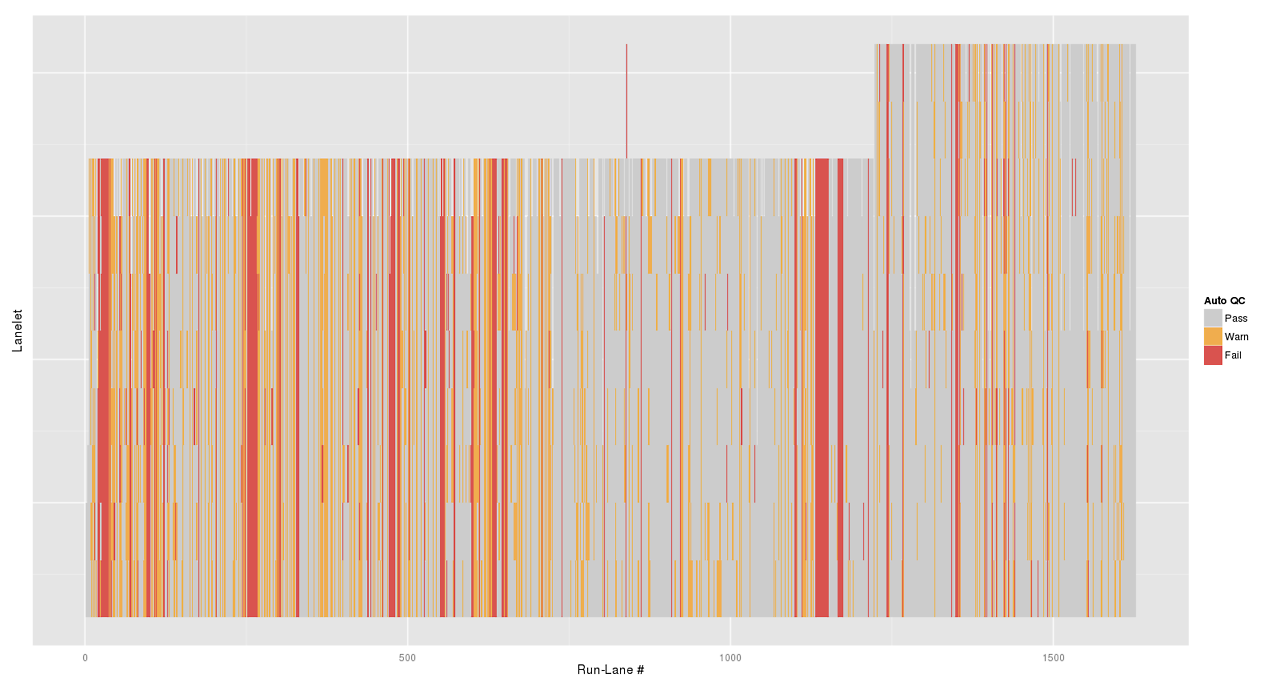
\includegraphics[width=1.0\textwidth]{classcorr}
    \caption[ClassCorr]{\textbf{Heatmap of lanelet QC status by lane}: Lanes are
    vertical bars with each lanelet cell coloured red to represent a failure,
yellow for a warning and grey for a pass.}
    \label{fig:classcorr}
\end{figure}

%TODO affected effected?
In such a case there would appear to exist a relationship between the respective
qualities of each lanelet in a lane as well as each lane in a sequencing run. To
examine this further, an R script utilising \textbf{ggplot2} was authored to
visually inspect whether correlation existed and if so to what degree that data
is affected.

Figure~\ref{fig:classcorr} displays a plot of \textbf{auto\_qc} classification
for each lanelet in a lane. The plot itself is a dense heatmap
where each lane stands as a vertical bar, broken in to horizontal cells, each
of which represents a lanelet that was sequenced in that particular lane. These
lanelets are colour coded using; red for failures, yellow for warnings and grey
for passes (to allow the other two classes to be more easily seen).

Therefore an unbroken vertical red line indicates that all lanelets that
comprise of that line failed to pass some aspect of the current
\textbf{auto\_qc} thresholds. In reality there are few conditions under which
a lanelet would fail irrespective of the status of the rest of the lanelets in
the same lane which typically involve an error during the preparation of the
sample (an easy to spot result as it will cause poor quality across all lanelets
using that sample).

%TODO Better explanation
Overall there are a series of instances appearing to support correlation for
whole-lane failures and warnings but despite this there do appear to be occasions
where a lanelet has failed where the remainder of the lane has not.
Having discussed this with the project supervisor and contacts at the Sanger Institute we decided to continue to
the implementation stage, agreeing that whilst some evidence of correlation
between lanelets in the same lane has emerged, we will still be able to recover
parameters that will be useful to quality control and statistical testing may be
required following this analysis to describe how powerful such parameters are
taking this possible correlation in to account.

It should be
noted that the proportion of failures and warnings is considerably smaller than
passes and so care will need to be taken to find a balance; for example it would
not be feasible to merely discard lanelets from lanes that have failed entirely
as there'd hardly be any data on which to train a classifier. Indeed other
solutions may be possible, perhaps weighting observations which exhibit similar
behaviour to other lanelets in their lane so as to give their parameter values
less priority during the construction of the classifier itself.

It is worth noting that although the plot does not make a particular
distinction between lanes in the same flow cell, lanes are sequentially
identified so the red bars of thicker-width arguably display some failures
across entire flow cells.

As a final note it should be stressed that this plot should be regarded as a
diagnostic rather than an experiment with a direct conclusion. Given more time it
would be useful to investigate the nature of these possible correlations, given
a lane that has failed across all lanelets: do those lanelets actually express
similar quality metrics?

%%%%%%%%%%%%%%%%%%%%%%%%%%%%%%%%%%%%%%%%%%%%%%%%%%%%%%%%%%%%%%%%%%%%%%%%%%%%%%%
\section{Recovering Ratios}

An initial scan of the summary numbers available in the "bamcheckr'd" files
introduced in Chapter~\ref{chap:bamcheckr-data} revealed 82 different
parameters. However, when comparing this parameter set to the threshold rules of
\textbf{auto\_qc}, it appeared that some parameters were "missing".

In the pursuit of replicating the decisions of the
existing system, it is ideal to have all the parameters used in the making of
those decisions at hand. In particular, the missing parameters were of a
normalised nature, typically in the form of a ratio or percentage which should
make them more valuable than a parameter that just represents a raw count of
some property.

It was found that these missing parameters are calculated in a step preceeding
\textbf{auto\_qc} as part of the \textbf{vr-pipe}
pipeline\footnote{https://github.com/wtsi-hgi/vr-pipe/blob/hgi-release/modules/VRPipe/Steps/vrtrack\_auto\_qc\_hgi\_3.pm}.

%...It is actually here that the hard-coded thresholds for warnings and failures
% are applied and the target decision is made too!

Whilst I could have attempted to set-up my own instance of \textbf{vr-pipe} to
recover this data, speaking with contacts at the Sanger Institute, it was
decided that this would prove troublesome work; requiring an involved
deployment to a cloud based facility such as Amazon's Elastic Compute Cloud and
installation of various Perl dependencies as well as requiring access to many
controlled databases within the institute.

Most of the functions that calculated these parameters turned out to be
straightforward and could easily be ported to another application. At first
it was intended to add these functions to the program authored for this part of
the project, but the Sanger Institute suggested it would be more useful to
implement such functionality in \textbf{bamcheckr} directly, removing some of
\textbf{auto\_qc}'s dependence on its position in \textbf{vr-pipe}.

\begin{listing}[H]
    \caption[r-dev]{: Installing an in-development R package with \textbf{devtools}}
    \label{list:r-dev}
    \begin{minted}[mathescape,
                %linenos,
                numbersep=5pt,
                gobble=8,
                frame=lines,
                framesep=2mm]{r}
        # Install and include the `devtools' package
        install.packages("devtools")
        library(devtools)

        # Install package directly from Github repository
        install_github("samstudio8/seq_autoqc", subdir="bamcheckr")

        # Install package from local directory
        install("/home/sam/Projects/seq_autoqc/bamcheckr")

    \end{minted}
\end{listing}

With the help of \textbf{devtools}\citep{man:devtools} (see
Listing~\ref{list:r-dev}) it was simple to develop and test contributions to
\textbf{bamcheckr} locally without needing to re-publish the package after
changes. An additional script was added to \textbf{bamcheckr}'s NAMESPACE... to
recover the missing ratio and percentage based parameters...

...unfortunately, the performance of the script was poor, taking 5.5s on average
and increasing to 16.1s when enabling a complex function containing many vector
operations (potentially inefficient due to my lack of R experience)...
for overlapping\_base\_duplicate\_percentage

...utilising the program designed and implemented in the following chapter...
loaded required information and used the API to calculate the missing
parameters...

...Morandat\citep{morandat-rperf}

%FUTURE
...with such an intriguing difference in performance with significantly more
time it would be appealing to explore the idiosyncrasies of each implementation
...although such an investigation would quite likely sufficiently generate an
entire project of its own.



%%%%%%%%%%%%%%%%%%%%%%%%%%%%%%%%%%%%%%%%%%%%%%%%%%%%%%%%%%%%%%%%%%%%%%%%%%%%%%%
\section{Contributions to bamcheckr}
...R CMD BATCH issue
...Fixed a graph plotting failure.

